% -----------------------
\subsection{Dekorationen}
% -----------------------
\begin{minipage}{0.7\textwidth}
  \footnotesize
  \input{decorationbent.code}
\end{minipage}\hfill
\begin{minipage}{0.29\textwidth}
  \centering
  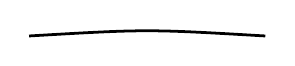
\begin{tikzpicture}[line width=1pt]
    % benoetigt \usetikzlibrary{decorations.pathmorphing}
    \draw[decorate, decoration=bent] (0, 0) -- (3, 0);
  \end{tikzpicture}
\end{minipage}

\begin{minipage}{0.7\textwidth}
  \footnotesize
  \input{decorationbumps.code}
\end{minipage}\hfill
\begin{minipage}{0.29\textwidth}
  \centering
  
\begin{tikzpicture}[line width=1pt]
    % benoetigt \usetikzlibrary{decorations.pathmorphing}
    \draw[decorate, decoration=bumps] (0, 0) -- (3, 0);
  \end{tikzpicture}
\end{minipage}

\begin{minipage}{0.7\textwidth}
  \footnotesize
  \input{decorationcoil.code}
\end{minipage}\hfill
\begin{minipage}{0.29\textwidth}
  \centering
  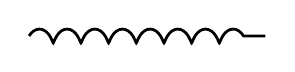
\begin{tikzpicture}[line width=1pt]
    % benoetigt \usetikzlibrary{decorations.pathmorphing}
    \draw[decorate, decoration=coil] (0, 0) -- (3, 0);
  \end{tikzpicture}
\end{minipage}

\begin{minipage}{0.7\textwidth}
  \footnotesize
  \input{decorationrandomsteps.code}
\end{minipage}\hfill
\begin{minipage}{0.29\textwidth}
  \centering
  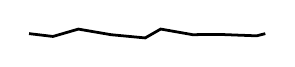
\begin{tikzpicture}[line width=1pt]
    % benoetigt \usetikzlibrary{decorations.pathmorphing}
    \draw[decorate, decoration=random steps] (0, 0) -- (3, 0);
  \end{tikzpicture}
\end{minipage}

\begin{minipage}{0.7\textwidth}
  \footnotesize
  \input{decorationsaw.code}
\end{minipage}\hfill
\begin{minipage}{0.29\textwidth}
  \centering
  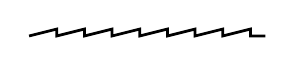
\begin{tikzpicture}[line width=1pt]
    % benoetigt \usetikzlibrary{decorations.pathmorphing}
    \draw[decorate, decoration=saw] (0, 0) -- (3, 0);
  \end{tikzpicture}
\end{minipage}

\begin{minipage}{0.7\textwidth}
  \footnotesize
  \input{decorationsnake.code}
\end{minipage}\hfill
\begin{minipage}{0.29\textwidth}
  \centering
  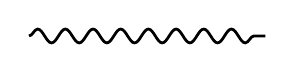
\begin{tikzpicture}[line width=1pt]
    % benoetigt \usetikzlibrary{decorations.pathmorphing}
    \draw[decorate, decoration=snake] (0, 0) -- (3, 0);
  \end{tikzpicture}
\end{minipage}

\begin{minipage}{0.7\textwidth}
  \footnotesize
  \input{decorationzigzag.code}
\end{minipage}\hfill
\begin{minipage}{0.29\textwidth}
  \centering
  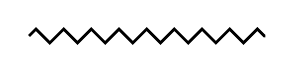
\begin{tikzpicture}[line width=1pt]
    % benoetigt \usetikzlibrary{decorations.pathmorphing}
    \draw[decorate, decoration=zigzag] (0, 0) -- (3, 0);
  \end{tikzpicture}
\end{minipage}

\begin{minipage}{0.7\textwidth}
  \footnotesize
  \input{decorationborder.code}
\end{minipage}\hfill
\begin{minipage}{0.29\textwidth}
  \centering
  \begin{tikzpicture}[line width=1pt]
    % benoetigt \usetikzlibrary{decorations.pathreplacing}
    \draw[decorate, decoration=border] (0, 0) -- (3, 0);
  \end{tikzpicture}
\end{minipage}

\begin{minipage}{0.7\textwidth}
  \footnotesize
  \input{decorationbrace.code}
\end{minipage}\hfill
\begin{minipage}{0.29\textwidth}
  \centering
  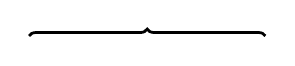
\begin{tikzpicture}[line width=1pt]
    % benoetigt \usetikzlibrary{decorations.pathreplacing}
    \draw[decorate, decoration=brace] (0, 0) -- (3, 0);
  \end{tikzpicture}
\end{minipage}

\begin{minipage}{0.7\textwidth}
  \footnotesize
  \input{decorationexpandingwaves.code}
\end{minipage}\hfill
\begin{minipage}{0.29\textwidth}
  \centering
  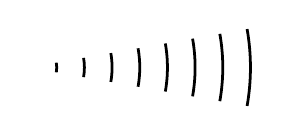
\begin{tikzpicture}[line width=1pt]
    % benoetigt \usetikzlibrary{decorations.pathreplacing}
    \draw[decorate, decoration={expanding waves, angle=10}]
         (0, 0) -- (3, 0);
  \end{tikzpicture}
\end{minipage}

\begin{minipage}{0.7\textwidth}
  \footnotesize
  \input{decorationticks.code}
\end{minipage}\hfill
\begin{minipage}{0.29\textwidth}
  \centering
  \begin{tikzpicture}[line width=1pt]
    % benoetigt \usetikzlibrary{decorations.pathreplacing}
    \draw[decorate, decoration=ticks] (0, 0) -- (3, 0);
  \end{tikzpicture}
\end{minipage}

\begin{minipage}{0.7\textwidth}
  \footnotesize
  \input{decorationwaves.code}
\end{minipage}\hfill
\begin{minipage}{0.29\textwidth}
  \centering
  \begin{tikzpicture}[line width=1pt]
    % benoetigt \usetikzlibrary{decorations.pathreplacing}
    \draw[decorate, decoration=waves] (0, 0) -- (3, 0);
  \end{tikzpicture}
\end{minipage}

\begin{minipage}{0.7\textwidth}
  \footnotesize
  \input{decorationcrosses.code}
\end{minipage}\hfill
\begin{minipage}{0.29\textwidth}
  \centering
  \begin{tikzpicture}[line width=1pt]
    % benoetigt \usetikzlibrary{decorations.shapes}
    \draw[decorate, decoration=crosses] (0, 0) -- (3, 0);
  \end{tikzpicture}
\end{minipage}

\begin{minipage}{0.7\textwidth}
  \footnotesize
  \input{decorationshapebackgrounds.code}
\end{minipage}\hfill
\begin{minipage}{0.29\textwidth}
  \centering
  \begin{tikzpicture}[line width=1pt]
    % benoetigt \usetikzlibrary{decorations.shapes}
    \draw[decorate, decoration=shape backgrounds]
         (0, 0) -- (3, 0);
  \end{tikzpicture}
\end{minipage}

\begin{minipage}{0.7\textwidth}
  \footnotesize
  \input{decorationtriangles.code}
\end{minipage}\hfill
\begin{minipage}{0.29\textwidth}
  \centering
  \begin{tikzpicture}[line width=1pt]
    % benoetigt \usetikzlibrary{decorations.shapes}
    \draw[decorate, decoration=triangles] (0, 0) -- (3, 0);
  \end{tikzpicture}
\end{minipage}

\begin{minipage}{0.7\textwidth}
  \footnotesize
  \input{decorationtextalongpath.code}
\end{minipage}\hfill
\begin{minipage}{0.29\textwidth}
  \centering
  \begin{tikzpicture}
    \clip (-3mm, -1mm) rectangle (28mm, 13mm);
    % benoetigt \usetikzlibrary{decorations.text}
    \draw[decorate, decoration={text along path,
                                text={abcdefghijklmnopqr}}]
         (0, 0) .. controls (1, 2) and (1, 0) .. (3, 0);
  \end{tikzpicture}
\end{minipage}

